A continuación mostramos los resultados obtenidos para el test de comparación entre factorización LU y eliminación gaussiana, los tiempos de cómputo se muestran en segundos y se usa escala logarítmica cuando es conveniente. Se muestran los resultados de matrices de 400x400, 225x225 y 100x100 


\begin{figure}[H]{}
\centering
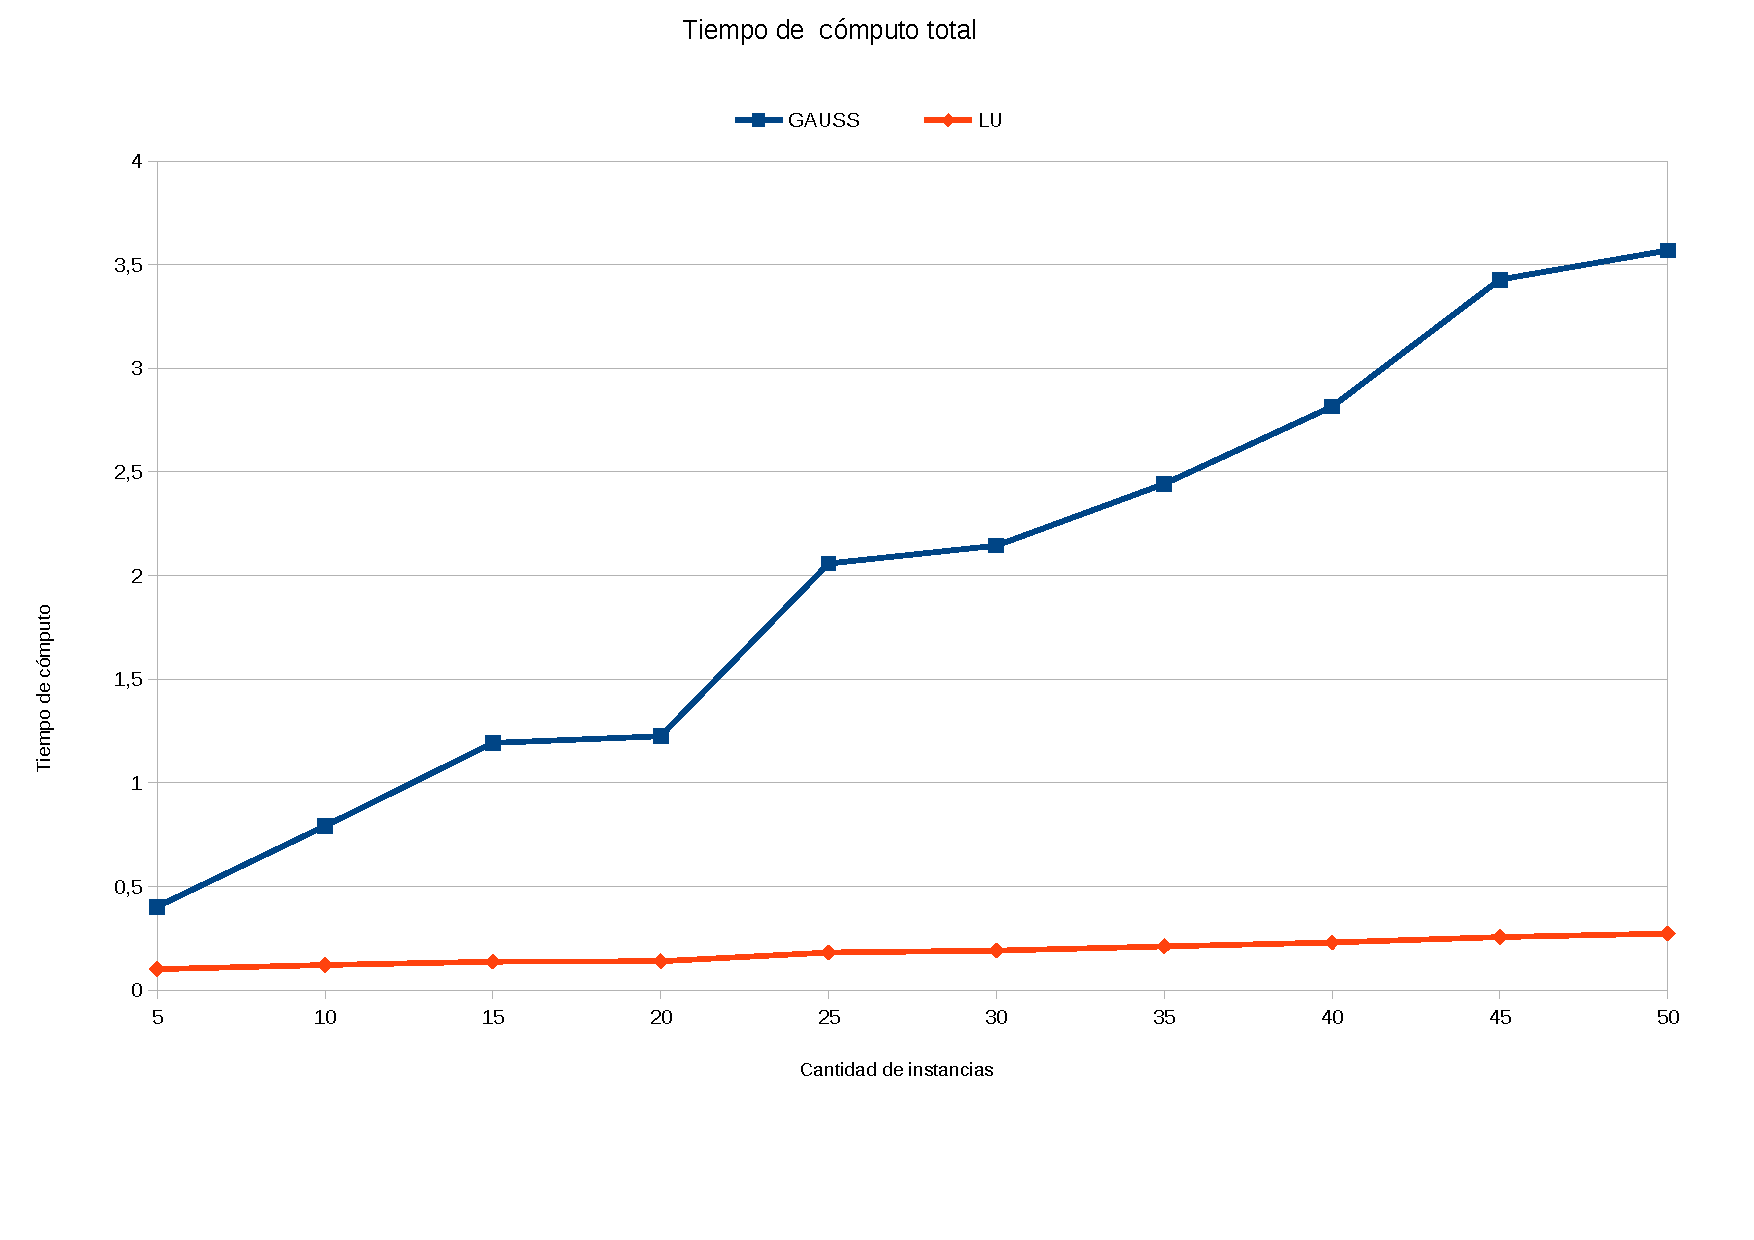
\includegraphics[scale=0.5]{graphs/gaussVsLU1.pdf}
\caption{Resultados obtenidos usando matrices de 20 ángulos y 20 radios. Se usa escala logarítmica.}
\label{gaussVsLU1}
\end{figure}

\begin{figure}[H]{}
\centering
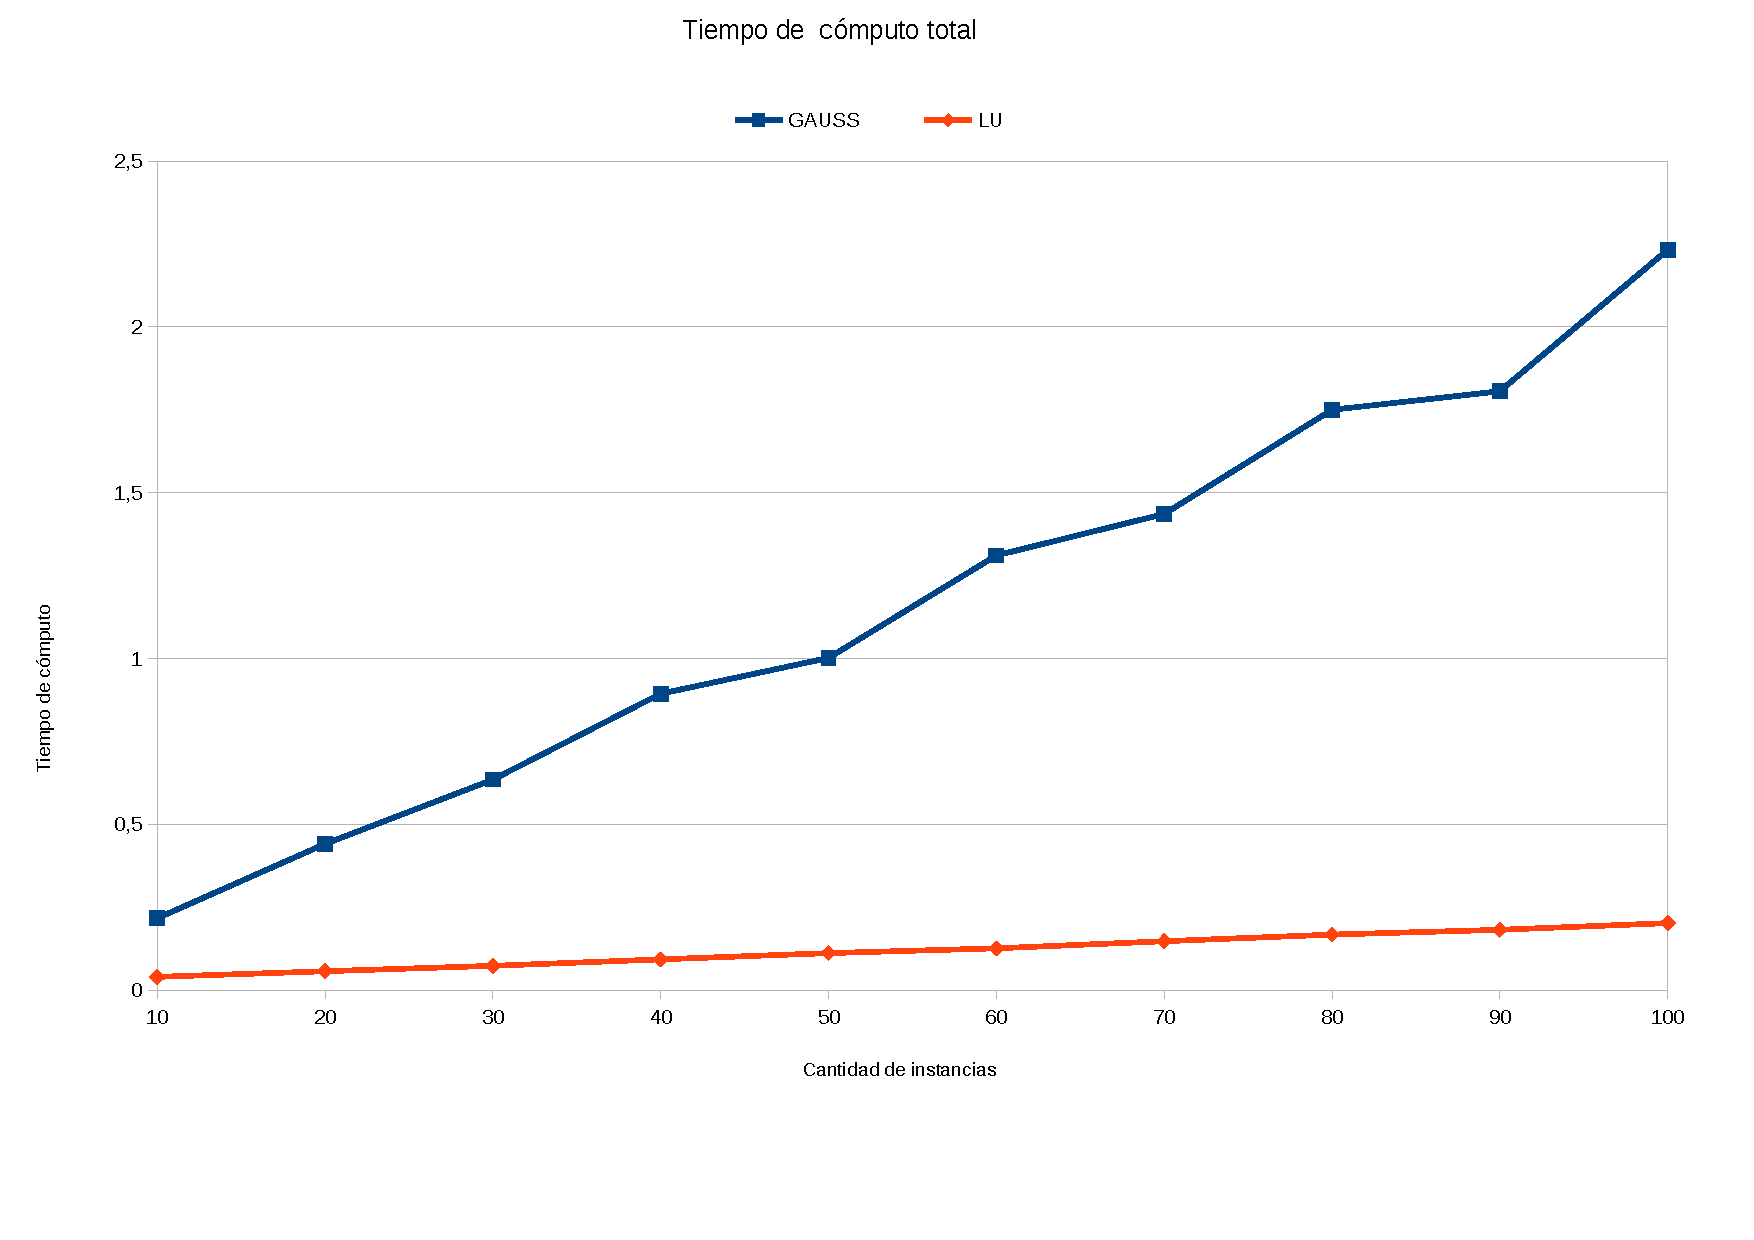
\includegraphics[scale=0.5]{graphs/gaussVsLU2.pdf}
\caption{Resultados obtenidos usando matrices de 15 ángulos y 15 radios. Se usa escala logarítmica.}
\label{gaussVsLU1}
\end{figure}

\begin{figure}[H]{}
\centering
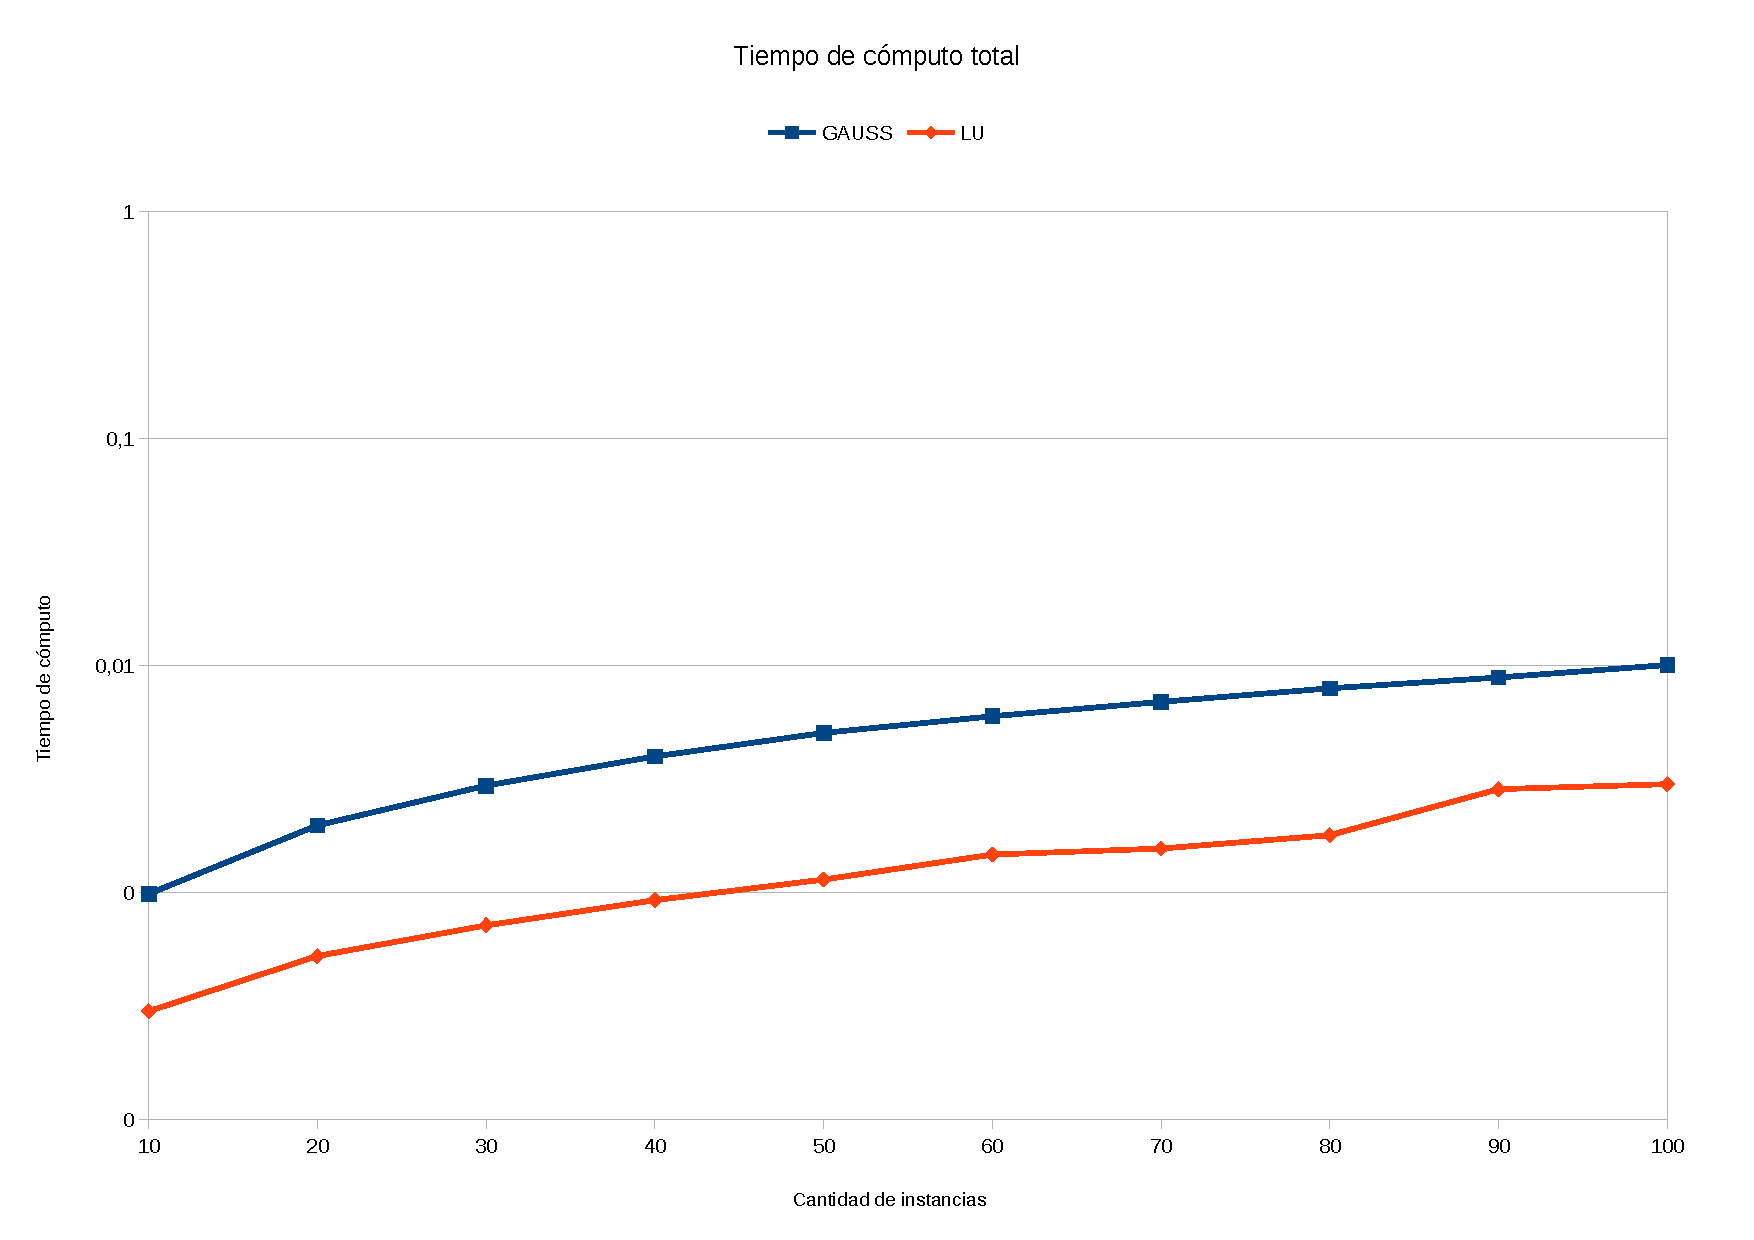
\includegraphics[scale=0.5]{graphs/gaussVsLU3.pdf}
\caption{Resultados obtenidos usando matrices de 10 ángulos y 10 radios. Se usa escala real.}
\label{gaussVsLU1}


\end{figure}
